\documentclass[12pt,]{article}
\usepackage[left=1in,top=1in,right=1in,bottom=1in]{geometry}
\newcommand*{\authorfont}{\fontfamily{phv}\selectfont}
\usepackage[]{libertine}


  \usepackage[T1]{fontenc}
  \usepackage[utf8]{inputenc}




\usepackage{abstract}
\renewcommand{\abstractname}{}    % clear the title
\renewcommand{\absnamepos}{empty} % originally center

\renewenvironment{abstract}
 {{%
    \setlength{\leftmargin}{0mm}
    \setlength{\rightmargin}{\leftmargin}%
  }%
  \relax}
 {\endlist}

\makeatletter
\def\@maketitle{%
  \newpage
%  \null
%  \vskip 2em%
%  \begin{center}%
  \let \footnote \thanks
    {\fontsize{18}{20}\selectfont\raggedright  \setlength{\parindent}{0pt} \@title \par}%
}
%\fi
\makeatother




\setcounter{secnumdepth}{0}

\usepackage{color}
\usepackage{fancyvrb}
\newcommand{\VerbBar}{|}
\newcommand{\VERB}{\Verb[commandchars=\\\{\}]}
\DefineVerbatimEnvironment{Highlighting}{Verbatim}{commandchars=\\\{\}}
% Add ',fontsize=\small' for more characters per line
\usepackage{framed}
\definecolor{shadecolor}{RGB}{248,248,248}
\newenvironment{Shaded}{\begin{snugshade}}{\end{snugshade}}
\newcommand{\AlertTok}[1]{\textcolor[rgb]{0.94,0.16,0.16}{#1}}
\newcommand{\AnnotationTok}[1]{\textcolor[rgb]{0.56,0.35,0.01}{\textbf{\textit{#1}}}}
\newcommand{\AttributeTok}[1]{\textcolor[rgb]{0.77,0.63,0.00}{#1}}
\newcommand{\BaseNTok}[1]{\textcolor[rgb]{0.00,0.00,0.81}{#1}}
\newcommand{\BuiltInTok}[1]{#1}
\newcommand{\CharTok}[1]{\textcolor[rgb]{0.31,0.60,0.02}{#1}}
\newcommand{\CommentTok}[1]{\textcolor[rgb]{0.56,0.35,0.01}{\textit{#1}}}
\newcommand{\CommentVarTok}[1]{\textcolor[rgb]{0.56,0.35,0.01}{\textbf{\textit{#1}}}}
\newcommand{\ConstantTok}[1]{\textcolor[rgb]{0.00,0.00,0.00}{#1}}
\newcommand{\ControlFlowTok}[1]{\textcolor[rgb]{0.13,0.29,0.53}{\textbf{#1}}}
\newcommand{\DataTypeTok}[1]{\textcolor[rgb]{0.13,0.29,0.53}{#1}}
\newcommand{\DecValTok}[1]{\textcolor[rgb]{0.00,0.00,0.81}{#1}}
\newcommand{\DocumentationTok}[1]{\textcolor[rgb]{0.56,0.35,0.01}{\textbf{\textit{#1}}}}
\newcommand{\ErrorTok}[1]{\textcolor[rgb]{0.64,0.00,0.00}{\textbf{#1}}}
\newcommand{\ExtensionTok}[1]{#1}
\newcommand{\FloatTok}[1]{\textcolor[rgb]{0.00,0.00,0.81}{#1}}
\newcommand{\FunctionTok}[1]{\textcolor[rgb]{0.00,0.00,0.00}{#1}}
\newcommand{\ImportTok}[1]{#1}
\newcommand{\InformationTok}[1]{\textcolor[rgb]{0.56,0.35,0.01}{\textbf{\textit{#1}}}}
\newcommand{\KeywordTok}[1]{\textcolor[rgb]{0.13,0.29,0.53}{\textbf{#1}}}
\newcommand{\NormalTok}[1]{#1}
\newcommand{\OperatorTok}[1]{\textcolor[rgb]{0.81,0.36,0.00}{\textbf{#1}}}
\newcommand{\OtherTok}[1]{\textcolor[rgb]{0.56,0.35,0.01}{#1}}
\newcommand{\PreprocessorTok}[1]{\textcolor[rgb]{0.56,0.35,0.01}{\textit{#1}}}
\newcommand{\RegionMarkerTok}[1]{#1}
\newcommand{\SpecialCharTok}[1]{\textcolor[rgb]{0.00,0.00,0.00}{#1}}
\newcommand{\SpecialStringTok}[1]{\textcolor[rgb]{0.31,0.60,0.02}{#1}}
\newcommand{\StringTok}[1]{\textcolor[rgb]{0.31,0.60,0.02}{#1}}
\newcommand{\VariableTok}[1]{\textcolor[rgb]{0.00,0.00,0.00}{#1}}
\newcommand{\VerbatimStringTok}[1]{\textcolor[rgb]{0.31,0.60,0.02}{#1}}
\newcommand{\WarningTok}[1]{\textcolor[rgb]{0.56,0.35,0.01}{\textbf{\textit{#1}}}}



\title{CSC8631 Coursework Assignment  }
 



\author{\Large Mariela Ayu Prasetyo
(210407835)\vspace{0.05in} \newline\normalsize\emph{Newcastle
University}  }


\date{}

\usepackage{titlesec}

\titleformat*{\section}{\normalsize\bfseries}
\titleformat*{\subsection}{\normalsize\itshape}
\titleformat*{\subsubsection}{\normalsize\itshape}
\titleformat*{\paragraph}{\normalsize\itshape}
\titleformat*{\subparagraph}{\normalsize\itshape}


\usepackage{natbib}
\bibliographystyle{apsr}
\usepackage[strings]{underscore} % protect underscores in most circumstances



\newtheorem{hypothesis}{Hypothesis}
\usepackage{setspace}


% set default figure placement to htbp
\makeatletter
\def\fps@figure{htbp}
\makeatother

\usepackage{hyperref}
\usepackage{array}
\usepackage{caption}
\usepackage{graphicx}
\usepackage{siunitx}
\usepackage{multirow}
\usepackage{hhline}
\usepackage{calc}
\usepackage{tabularx}
\usepackage{fontawesome}
\usepackage[para,online,flushleft]{threeparttable}

% move the hyperref stuff down here, after header-includes, to allow for - \usepackage{hyperref}

\makeatletter
\@ifpackageloaded{hyperref}{}{%
\ifxetex
  \PassOptionsToPackage{hyphens}{url}\usepackage[setpagesize=false, % page size defined by xetex
              unicode=false, % unicode breaks when used with xetex
              xetex]{hyperref}
\else
  \PassOptionsToPackage{hyphens}{url}\usepackage[draft,unicode=true]{hyperref}
\fi
}

\@ifpackageloaded{color}{
    \PassOptionsToPackage{usenames,dvipsnames}{color}
}{%
    \usepackage[usenames,dvipsnames]{color}
}
\makeatother
\hypersetup{breaklinks=true,
            bookmarks=true,
            pdfauthor={Mariela Ayu Prasetyo (210407835) (Newcastle
University)},
             pdfkeywords = {},  
            pdftitle={CSC8631 Coursework Assignment},
            colorlinks=true,
            citecolor=blue,
            urlcolor=blue,
            linkcolor=magenta,
            pdfborder={0 0 0}}
\urlstyle{same}  % don't use monospace font for urls

% Add an option for endnotes. -----


% add tightlist ----------
\providecommand{\tightlist}{%
\setlength{\itemsep}{0pt}\setlength{\parskip}{0pt}}

% add some other packages ----------

% \usepackage{multicol}
% This should regulate where figures float
% See: https://tex.stackexchange.com/questions/2275/keeping-tables-figures-close-to-where-they-are-mentioned
\usepackage[section]{placeins}


\begin{document}
	
% \pagenumbering{arabic}% resets `page` counter to 1 
%    

% \maketitle

{% \usefont{T1}{pnc}{m}{n}
\setlength{\parindent}{0pt}
\thispagestyle{plain}
{\fontsize{18}{20}\selectfont\raggedright 
\maketitle  % title \par  

}

{
   \vskip 13.5pt\relax \normalsize\fontsize{11}{12} 
\textbf{\authorfont Mariela Ayu Prasetyo
(210407835)} \hskip 15pt \emph{\small Newcastle University}   

}

}






\vskip -8.5pt


 % removetitleabstract

\noindent  

\hypertarget{introduction}{%
\section{Introduction}\label{introduction}}

This report aims to discuss and report any findings to the CSC8631
coursework assignment regarding exploratory data analysis in learning
analytics. Regarding the data set, the students were provided with one
from FutureLearn MOOC. We are then asked to provide any valuable or
non-valuable insights while following the best-practice development
explained thoroughly via the teaching resources available. To ensure we
are following the data-driven process throughout the project, we will
also be adhering to the CRISP-DM methodology. Lastly, we will wrap up
with a conclusion regarding the overall findings.

\hypertarget{business-understanding}{%
\section{Business Understanding}\label{business-understanding}}

The first step of CRISP-DM is the \emph{Business Understanding} step,
where we try to understand what the business wants to solve. In this
particular project, we are given the data set regarding a course in the
FutureLearn MOOC platform. Just like a real-life face-to-face class, we
want to find out whether students are involved in the class or not and
how many students continue to participate until the end of the semester.
We are also interested in finding out how many students leave the class
and, naturally, their reason for doing so. Lastly, we want our course to
improve constantly, so we will consider any feedback from the data
(CHECK). Formulating all of the previous problems into a sentence, we
come up with the following precise questions :

\begin{itemize}
\tightlist
\item
  What is the participation rate of the students? (CHECK): and Are there
  any variables closely related to this?
\item
  How many students and what causes students to leave the course?
\item
  Which part of the learning course can we further improve?
\end{itemize}

\hypertarget{data-understanding-and-data-preparation}{%
\section{Data Understanding and Data
Preparation}\label{data-understanding-and-data-preparation}}

After formulating the questions, we move on to the \emph{Data
Understanding} and \emph{Data Preparation} part, where we focus on
understanding and formatting the data that assist the business tasks
defined in \emph{Business Understanding}. This phase will consist of:

\begin{itemize}
\item
  Describe data: In this part, we are trying to understand and describe
  the data in a short description. We can do this by examining the data
  format, the number of rows and columns, and the features that are
  accessible.
\item
  Exploring the data: In this section, we are trying to analyse the
  relationship between data and visualise the data. The conclusion and
  visualisation of the data exploration should support and verify the
  business question defined previously. We will also select, clean,
  integrate and formatting the data for easier visualisation and
  modeling (CHECK)
\end{itemize}

\hypertarget{describe-data}{%
\subsection{Describe Data}\label{describe-data}}

Firstly, we are given the data set regarding an online course from the
FutureLearn MOOC platform. The data set consists of several files for
each run from run 1 to run 7. Each run may consist of the following data
in the .csv form (the number inside the bracket denotes how many
variables are there in the file):

\begin{itemize}
\tightlist
\item
  archetype survey response (4)
\item
  enrolments (13)
\item
  leaving survey response (8)
\item
  question response (10)
\item
  step activity (6)
\item
  team members (5)
\item
  video stats (28)
\item
  weekly sentiment survey response (4)
\end{itemize}

Each of the files consists of different rows (entries), and all the
columns (variables) are stored in a chr format.

\hypertarget{exploring-the-data}{%
\subsection{Exploring the Data}\label{exploring-the-data}}

In this section, we will begin to explore the given data set. In
particular, we want to explore the area where the solution will support
the problem defined in the \emph{Business Understanding} part. There are
three questions and we will explore them one by one.

\hypertarget{question-1}{%
\subsubsection{Question 1}\label{question-1}}

\textbf{What is the participation rate of the students? (CHECK): and Are
there any variables closely related to this?}\\
\hfill\break For the first question, we want to analyse whether students
are highly engaged in the course. There are many ways to check this, but
we will focus on how many percentages of students fully participated and
finished the material of the classes. Additionally, we will also check
the duration of the completion for each student. \hfill\break We can do
this by checking the enrolments.csv provided in the data set. First, we
will do some data pre-processing.

\begin{Shaded}
\begin{Highlighting}[]
\CommentTok{\#read file enrolments run 1 to 7}
\NormalTok{files }\OtherTok{=} \FunctionTok{list.files}\NormalTok{(}\AttributeTok{path =} \StringTok{"data/"}\NormalTok{, }
                   \AttributeTok{pattern=}\StringTok{"*enrolments.csv"}\NormalTok{, }\AttributeTok{full.names =}\NormalTok{ T)}

\CommentTok{\#store each run in a single variable}
\ControlFlowTok{for}\NormalTok{ (i }\ControlFlowTok{in} \DecValTok{1}\SpecialCharTok{:}\FunctionTok{length}\NormalTok{(files)) \{}
\NormalTok{  temp }\OtherTok{\textless{}{-}} \FunctionTok{paste}\NormalTok{(}\StringTok{"enrolments"}\NormalTok{, i, }\AttributeTok{sep =} \StringTok{""}\NormalTok{)}
  \FunctionTok{assign}\NormalTok{(temp, }\FunctionTok{read.csv}\NormalTok{(files[i]))}
\NormalTok{\}}
\end{Highlighting}
\end{Shaded}

We read and store each run of enrolments in a single variable for a
later use. After that, we begin to do some processing in our data. We
begin by subsetting the students who fully participated in the course
(there are entries for the fully\_participated columns in the csv data).

\begin{Shaded}
\begin{Highlighting}[]
\NormalTok{enrolments }\OtherTok{\textless{}{-}} 
\NormalTok{  enrolments[}\SpecialCharTok{!}\NormalTok{enrolments}\SpecialCharTok{$}\NormalTok{fully\_participated\_at }\SpecialCharTok{==} \StringTok{""}\NormalTok{ , ]}
\end{Highlighting}
\end{Shaded}

Then, we convert the enrolled\_at and fully\_participated variables of
each run from string format to date format to calculate the duration
later on. We convert it by using the as.Date function.

\begin{Shaded}
\begin{Highlighting}[]
\FunctionTok{as.Date}\NormalTok{(}\FunctionTok{as.character}\NormalTok{(enrolments\_na}\SpecialCharTok{$}\NormalTok{enrolled\_at), }
        \AttributeTok{format =} \StringTok{"\%Y{-}\%m{-}\%d"}\NormalTok{) }
\FunctionTok{as.Date}\NormalTok{(}\FunctionTok{as.character}\NormalTok{(enrolments\_na}\SpecialCharTok{$}\NormalTok{fully\_participated\_at), }
        \AttributeTok{format =} \StringTok{"\%Y{-}\%m{-}\%d"}\NormalTok{)}
\end{Highlighting}
\end{Shaded}

After converting it, we calculate the duration between the
fully\_participated\_at and enrolled\_at and store it in a new variable.
We also remove entries or outliers for each run where the period exceeds
365 days or one year.

\begin{Shaded}
\begin{Highlighting}[]
\NormalTok{enrolments1\_na }\OtherTok{\textless{}{-}}\NormalTok{ enrolments1\_na[}\SpecialCharTok{!}\NormalTok{(enrolments1\_na}\SpecialCharTok{$}\NormalTok{duration }
                                   \SpecialCharTok{\textgreater{}} \DecValTok{365}\NormalTok{) , ]}
\end{Highlighting}
\end{Shaded}

Lastly, we calculate the percentage of students who fully participated
in the course proportion to the overall enrollment for each run.

\begin{Shaded}
\begin{Highlighting}[]
\NormalTok{enrolments\_completion\_rate[}\DecValTok{1}\NormalTok{] }\OtherTok{=} 
  \FunctionTok{dim}\NormalTok{(enrolments1\_na)[}\DecValTok{1}\NormalTok{]}\SpecialCharTok{/}\FunctionTok{dim}\NormalTok{(enrolments1)[}\DecValTok{1}\NormalTok{] }\SpecialCharTok{*} \DecValTok{100}
\end{Highlighting}
\end{Shaded}

After preparing all of the data, we can now do the graphing. For the
first graph, we will graph using ggplot2 the duration of completion
against the starting date for each student in each run.

\begin{Shaded}
\begin{Highlighting}[]
\CommentTok{\# Insert plot}
\NormalTok{graph1}
\end{Highlighting}
\end{Shaded}

\begin{center}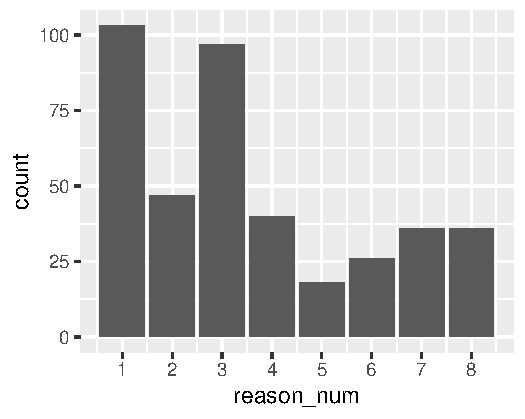
\includegraphics{report_files/figure-latex/unnamed-chunk-7-1} \end{center}

For the second graph, we will include the percentage of students who
fully participated in the course proportion to the overall enrollment
for each run.

\begin{Shaded}
\begin{Highlighting}[]
\CommentTok{\# Insert plot}
\NormalTok{graph2}
\end{Highlighting}
\end{Shaded}

\begin{center}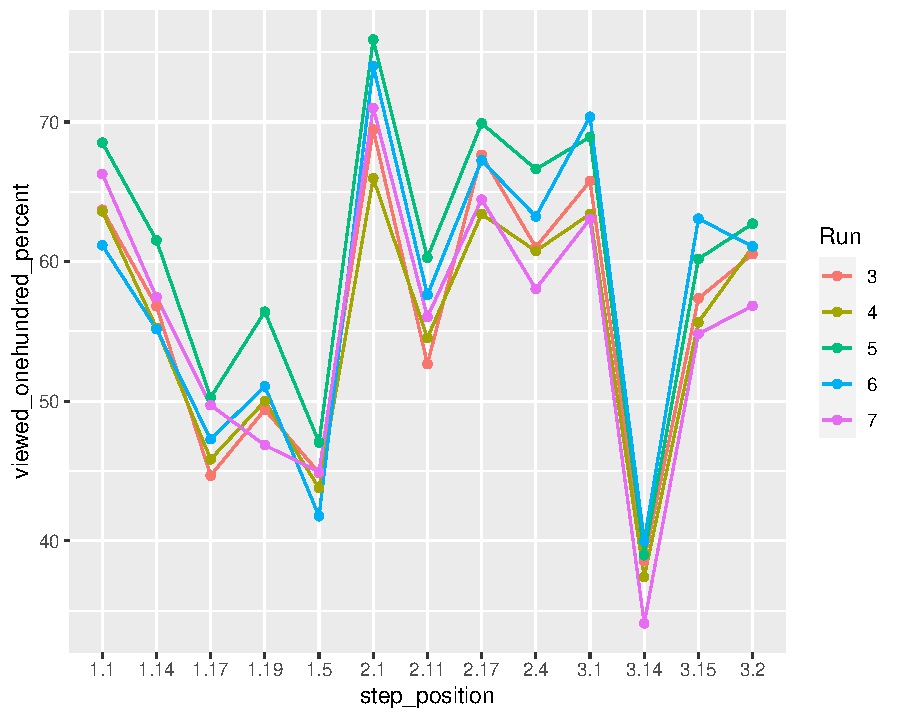
\includegraphics{report_files/figure-latex/unnamed-chunk-8-1} \end{center}

\emph{Discussion}

In graph 1, we can see that duration of students completing the courses
vary, but mostly concentrated in 0 to 150 days

\hypertarget{question-2}{%
\subsubsection{Question 2}\label{question-2}}

\textbf{How many students and what causes students to leave the course?}

\hypertarget{question-3}{%
\subsubsection{Question 3}\label{question-3}}

\textbf{Which part of the learning course can we further improve?}

\hypertarget{additional-notes}{%
\subsubsection{Additional notes}\label{additional-notes}}

Configuration setting, when





\newpage
\singlespacing 
\bibliography{master.bib}

\end{document}